% !TeX spellcheck = en_GB
\documentclass[10pt,a4paper]{article}
\usepackage[latin1]{inputenc}
\usepackage{color}
\usepackage{graphicx} %pictures
\usepackage{listings} %code
%setup for code
\lstset{
numbers=left,  % where to put the line-numbers
numbersep=5pt, % how far the line-numbers are from the code
}

\title{Finding the Convex Hull with Application to Distance Measurements for a Formula Student Car}
\author{Benedikt Schlereth}
\date{\today}

\begin{document}
	\maketitle
	\tableofcontents
	\pagebreak
	
	\begin{abstract}
	To find cones on the track for autonomous racing a computer has to visualize them and know how far away they are.
	For Visualizing the features of the cones inside the image are filtered out. After extracting the color the contours have rough edges. To smooth them out the convex hull gives back a nice contour with the out-most boundary of the cones. Knowing the dimension of the cone and proportions a Distance estimation can be done.
	\end{abstract}
	
	\section{Introduction}
	Formula-Student is an international design and construction competition where teams from all around the world are constructing and then racing single seat formula race-cars. With	the new event of Formula-Student-Driver-less Teams are encouraged to develop their own self-Driving cars. My motivation is to kick-offthe development of our own Driver-less Vehicle by implementing the rst step and providing a way to detect the boundaries of a race track. The tracklayout 
	
	\section{Steps to extract the features}
	To find the cones inside a picture one could create a dataset of 100+ cones and then train a neural network. But working with a neural network brings the additional difficulties to choose a network type that is efficient to run on a mobile platform while being reliable.
	It is also not necessary for this type of application to detect different objects in one frame.
	With only cones in three different colors to detect it is quite simple to describe the features of them.
	To visualize the process i choose a scene with green cones an different lighting and ground.
	\begin{figure}[h]
		\centering
		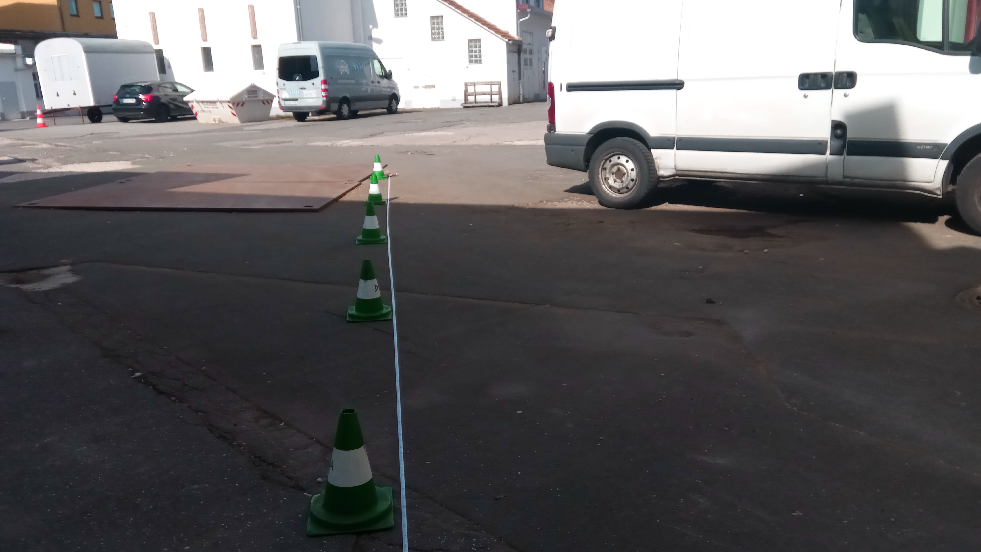
\includegraphics[width=0.5\textwidth]{Abb/start.png}
		\caption{example image}
		\label{example image}
	\end{figure}
	The picture is taken from a height of $1,2 m$ and the distance between the cones is $2m$ with the nearest $2m$ and the farthest $10m$ away from the camera.
	 
	\subsection{color filtering}
	The most obvious feature is the color. So the first step is to implement a colorfilter.
	\begin{lstlisting}[language=Python]
hsv = cv2.cvtColor(image, cv2.COLOR_BGR2HSV)
	
# value for colorfilter
lower_green = np.array([30, 100, 0])
upper_green = np.array([90, 255, 255])
	
mask = cv2.inRange(hsv, lower_green, upper_green)
res = cv2.bitwise_and(hsv, hsv, mask=mask)

blur = cv2.GaussianBlur(res, (15, 15), 0)
return blur, mask
	\end{lstlisting}
	The image provided for the colorfilter needs to be converted from the RGB values to the HSV colorspace.
	The HSV describes the color not with an eight-Bit value for red, green and blue but with a circle where the first value is for the color with 0 beeing red and 255 blue.
	The second value is needed for the saturation and the third and last value describes how bright the color will be represented.
	
	With knowing how the HSV-colorspace works it is possible to find the right values which will describe the color of our cones. It will be necessary to try the colorfilter for images in bright sunlight as well as cloudy conditions the make sure to be able to detect cones in every possible environment.
	
	Next up is comparing every Pixel with our given value. With the OpenCV function "inRange" one image will be read and compared to our boundaries. It returns a binary image which means everywhere the color was in Range a one is remaining and everywhere else a zero.
	
	\subsection{contours}
	After the Color-filter we are left with a binary image. Now it is quit easy to detect the edges of where it changes from black to white.
	
	\begin{figure}[h]
		\centering
		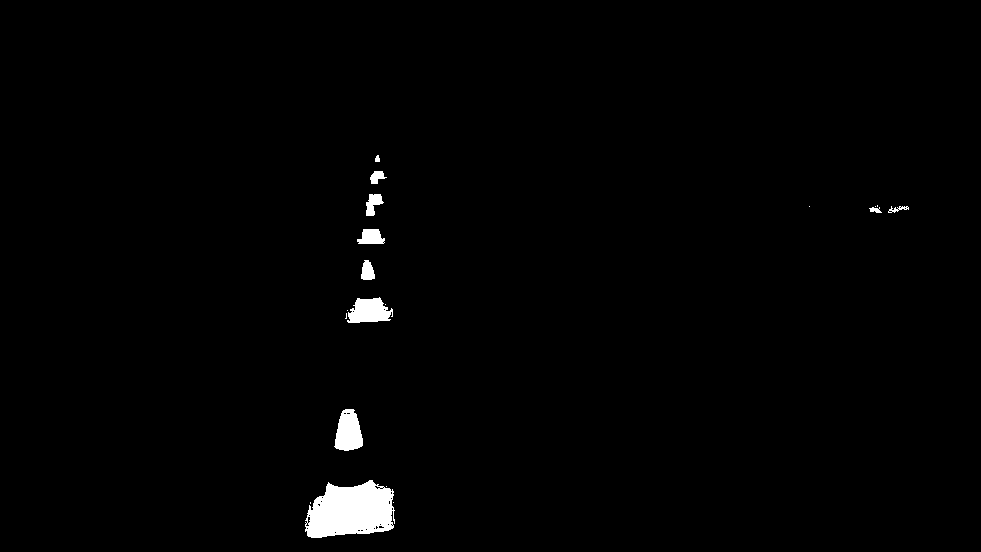
\includegraphics[width=0.5\textwidth]{Abb/mask.png}
		\caption{binary-image}
		\label{binary-image}
	\end{figure}
	
	But as seen in the top right hand corner of the image some noise will be left inside the picture. Therefore another filter is needed. A good difference between important and noisy areas is the size of the contour. This will delete all small contours which are most probably not important but also cones that are far away. The first test showed that excluding such cones does not matter.
	
	\subsection{hierarchy}
	Sometimes small dots or areas are left inside on parts of the cones. Luckily the contour-function gives us back the hierarchy of the contours. By filtering out the smaller regions inside the bigger ones no leaves only parts of the cones with no noise inside the areas.
	
	\subsection{convex-hull}
	The next step will be to find the convex hulls. What those are and how they are found will be described in the section \ref{convex-hull}. The convex-hull leaves a very good approximation of the cones edges as seen in Figure \ref{convex-hull-picture}
	\begin{figure}[h]
		\centering
		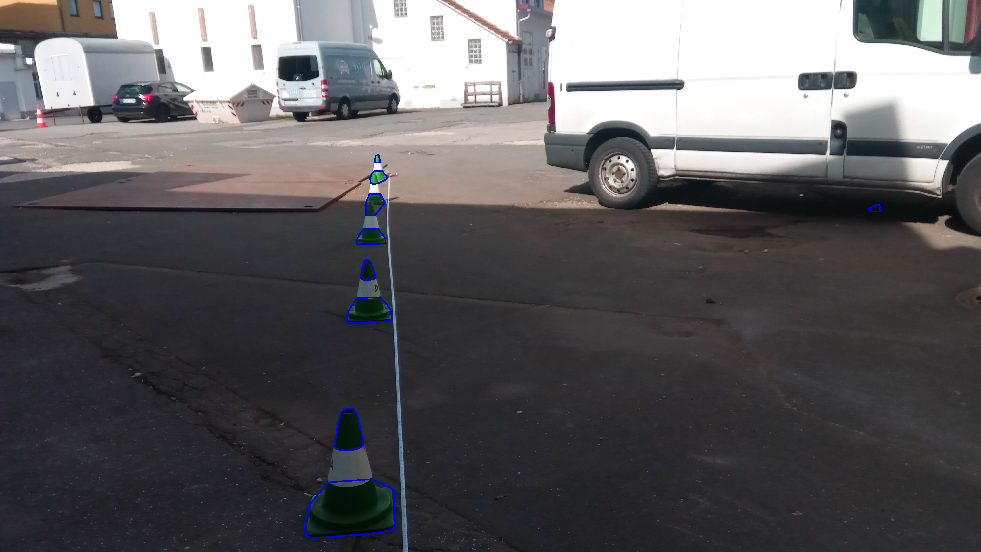
\includegraphics[width=0.5\textwidth]{Abb/convex-hull.png}
		\caption{convex-hull}
		\label{convex-hull-picture}
	\end{figure}
	
	\subsection{aspect ratio}
	A nice feature of the cones is the round top part. So no matter at what angle or distance the convex hull is detected the ratio between the height and width stays the same.
	
	\subsection{bounding box}
	With every top part of the cones found now the bottom part needs to be added. Therefore the distance to every other contour is calculated and the nearest one below the top part belongs to the same cone.
	The maximum points of both contours give the outlines of a bounding box which is drawn with red-color in Figure \ref{bounding-box}
	
	\begin{figure}[h]
		\centering
		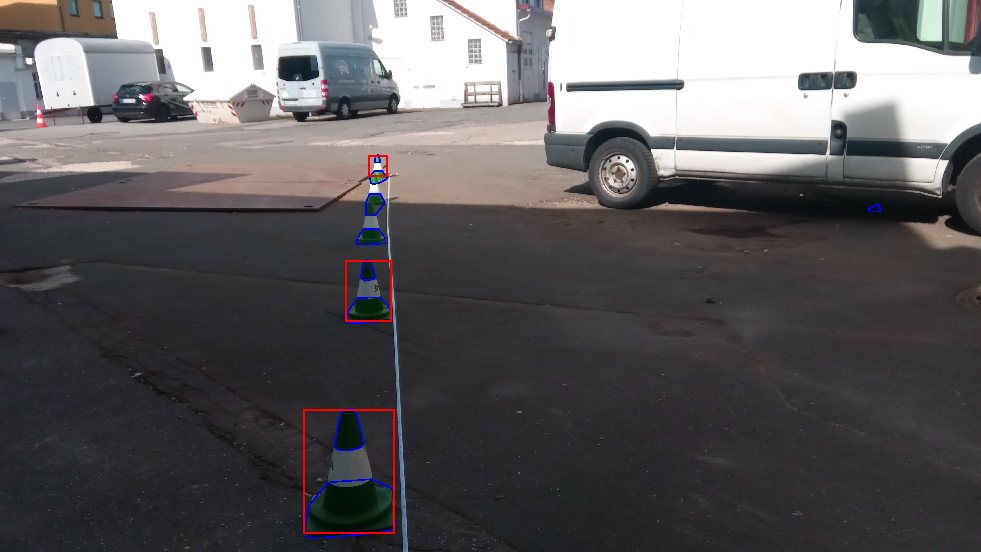
\includegraphics[width=0.5\textwidth]{Abb/bounding-box.png}
		\caption{bounding-box}
		\label{bounding-box}
	\end{figure}
	
	\section{convex-Hull algorithm by Graham} \label{convex-hull}
	
	\section{distance estimation}
	To find out where the cones are on the track the distance to each cone must be calculated. 
	With only one camera the number of pixel is the only value that can be used. 
	A stereo camera on the other hand would make triangulation possible.

	\subsection{Height}
	% estimate the distance with the pixel in vertical direction 
	
	\subsection{ratio}
	% estimate distance with the distance between the top and bottom part of the cone
	
	\subsection{error}
	% estimate the error of the calculation
	
	\subsection{disruption}
	% discuss possible disruptions that can occur while driving (e.g bumps on the track)
	
	\section{tests}
	% test the algorithmus with different lighting and roadcondition
	
	\section{summary}
	% Discussion after evaluating the tests
	
	\section{discussion}
	% Steps in the future (e.g draw own pictures to test faulty inputs, test robustness of code)
	
\end{document}